% ── Title slide ──────────────────────────────────────────────────────────────
\begin{frame}
  \titlepage
\end{frame}

% ── Who uses PyTorch? ─────────────────────────────────────────────────────────
\begin{frame}{}
  \centering
  \Huge Who uses PyTorch here?
\end{frame}

% ── Looks familiar? ───────────────────────────────────────────────────────────
\begin{frame}{Looks familiar?}
  \centering
  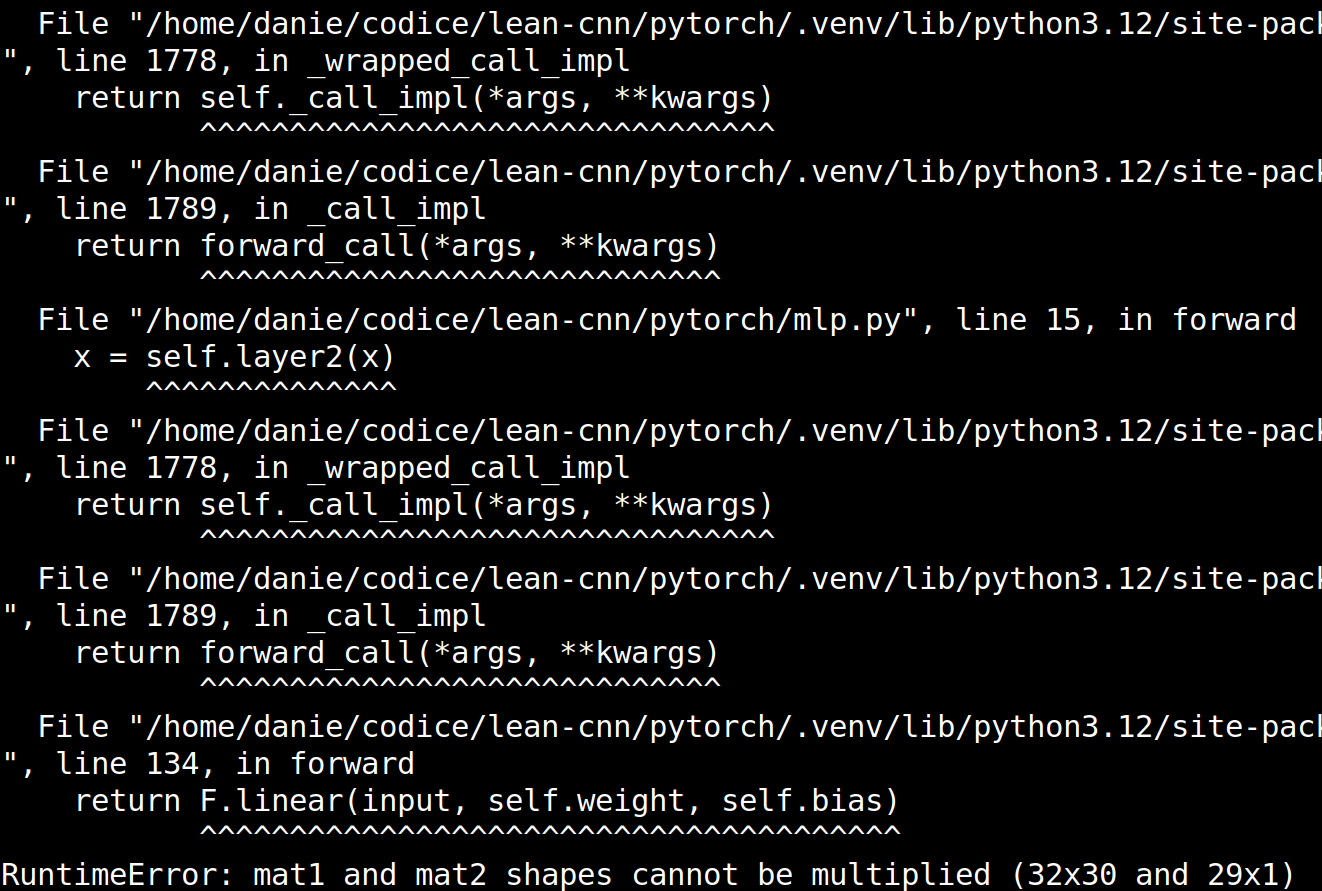
\includegraphics[width=\linewidth,height=0.82\textheight,keepaspectratio]{imgs/pytorch failure.png}
\end{frame}

% ── No more ───────────────────────────────────────────────────────────────────
\begin{frame}{}
  \centering
  \textbf{no more with fully typed neural networks}

  \vspace{0.5em}

  \begin{columns}[c]
    \begin{column}{0.65\textwidth}
      
\includegraphics[width=\linewidth,height=0.65\textheight,keepaspectratio]{imgs/torch lean website.png}

      \vspace{0.3em}
      \footnotesize\url{https://lean-dojo.github.io/TorchLean/}
    \end{column}
    \begin{column}{0.32\textwidth}
      
\includegraphics[width=\linewidth,height=0.72\textheight,keepaspectratio]{imgs/lowcortisol.png}
    \end{column}
  \end{columns}
\end{frame}

% ── What is Lean? ─────────────────────────────────────────────────────────────
\begin{frame}{What is Lean?}
  \begin{itemize}
    \item Functional programming language and interactive theorem prover
    \item Every expression has a precise type — the compiler is also a proof checker
    \item Dependent types let you encode invariants directly in the type system
    \item Developed at AWS and Microsoft Research; used in formal mathematics (Mathlib)
    \item Growing ecosystem for verified, type-safe scientific computing
  \end{itemize}
  \vfill
  \footnotesize\url{https://lean-lang.org/}
\end{frame}

% ── What is TorchLean? ───────────────────────────────────────────────────────
\begin{frame}{TorchLean}
  \begin{itemize}
    \item A Lean library providing access to PyTorch functionality
    \item Lives inside Lean's strong type system — with strong static guarantees
    \item No way to code a network with incompatible layers: shape errors caught at compile time
    \item Many more guarantees on the software: memory safety, totality, and formal correctness
  \end{itemize}
  \vfill
  \centering
  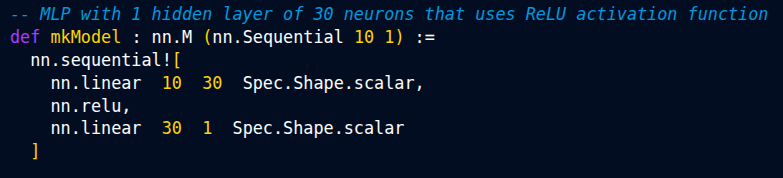
\includegraphics[width=\linewidth,height=0.45\textheight,keepaspectratio]{imgs/torchlean mlp.png}
\end{frame}

% ── Lean gets it ─────────────────────────────────────────────────────────────
\begin{frame}{Lean gets it}
  \centering
  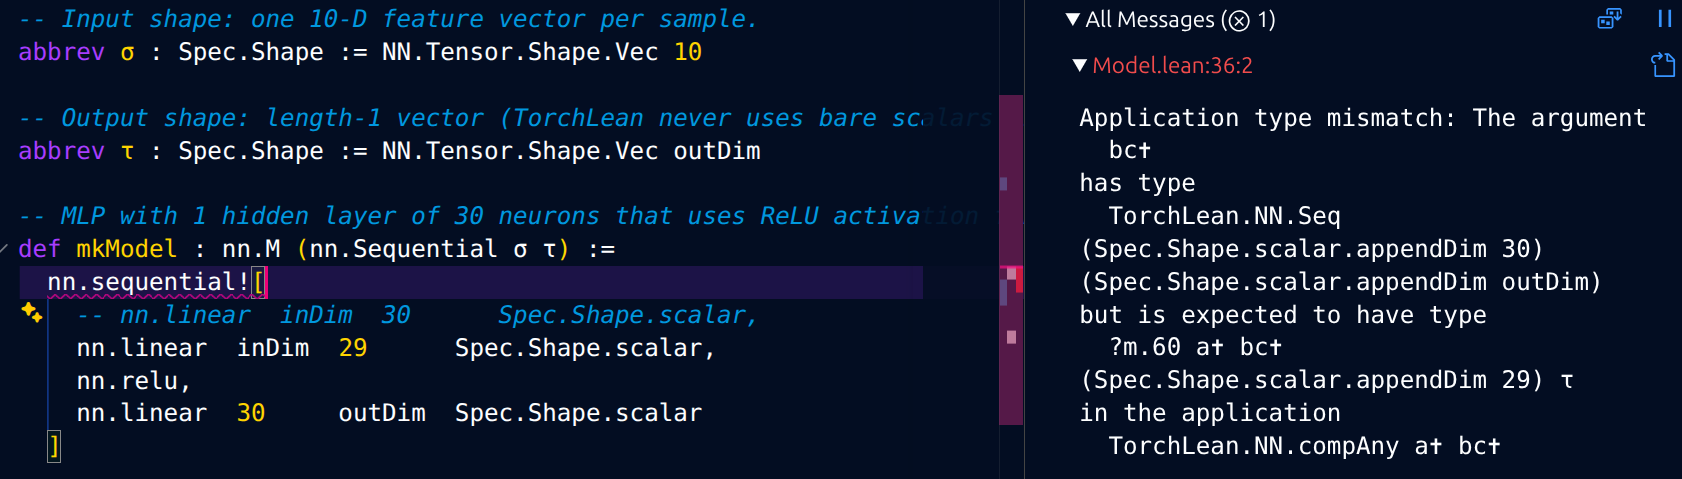
\includegraphics[width=\linewidth,height=0.82\textheight,keepaspectratio]{imgs/lean error.png}
\end{frame}

% ── Despite annotations ──────────────────────────────────────────────────────
\begin{frame}{}
  \centering
  \textbf{despite annotations this will always compile, run, and fail}

  \vfill
  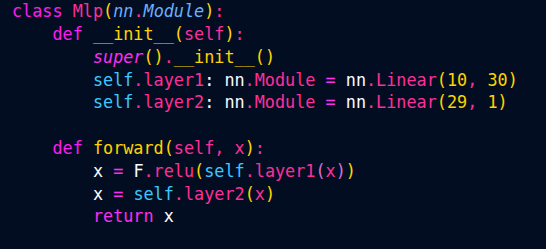
\includegraphics[width=\linewidth,height=0.75\textheight,keepaspectratio]{imgs/pytorch annotated.png}
\end{frame}

% ── Soyjak ───────────────────────────────────────────────────────────────────
\begin{frame}{}
  \begin{columns}[c]
    \begin{column}{0.45\textwidth}
      \centering
      
\includegraphics[width=\linewidth,height=0.82\textheight,keepaspectratio]{imgs/soyjak.jpg}
    \end{column}
    \begin{column}{0.50\textwidth}
      \large
      ``but annotations are annoying and useless
      i dont want to write them
      and duck typing is so convenient because flexibility
      or whatever''
    \end{column}
  \end{columns}
\end{frame}

% ── Big duck propaganda ───────────────────────────────────────────────────────
\begin{frame}{Big duck propaganda!}
  \begin{itemize}
    \item Useless annotations have been solved since the 70s, but Java wasn't paying attention\\
          (see ML, Rust, TypeScript, Kotlin\ldots)
    \item Structural type systems allow for ``if it quacks like a duck\ldots'' typing\\
          (again, see TypeScript)
  \end{itemize}
\end{frame}

% ── Back to reality ───────────────────────────────────────────────────────────
\begin{frame}{Back to reality}
  \begin{itemize}
    \item I'm not seriously advocating for using Lean to code neural networks
    \item However, stronger and flexible type systems are possible
    \item A man can hope for a TypeScript-like revolution for Python (and PyTorch!)
  \end{itemize}
\end{frame}

% ── Bottom line ───────────────────────────────────────────────────────────────
\begin{frame}{Bottom line}
  \begin{columns}[c]
    \begin{column}{0.28\textwidth}
      \centering
      \Large\textbf{static typing: awesome}
    \end{column}
    \begin{column}{0.40\textwidth}
      \centering
      
\includegraphics[width=\linewidth,height=0.72\textheight,keepaspectratio]{imgs/lowcortisol.png}
    \end{column}
    \begin{column}{0.28\textwidth}
      \centering
      \Large\textbf{dynamic typing: stinks}
    \end{column}
  \end{columns}
\end{frame}

% ── Closing ───────────────────────────────────────────────────────────────────
\begin{frame}{}
  \centering
  \Huge rant over
\end{frame}
